\section{block ciphers}
\begin{frame}
	\frametitle{block ciphers}
	block ciphers encrypt plaintext of a fixed length (64 bit and 128 bit are quite common)
	\begin{figure}
	 \begin{minipage}[b]{.4\linewidth}
		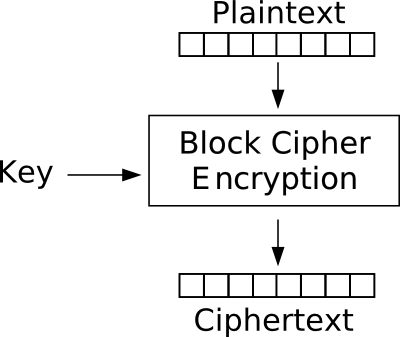
\includegraphics[width=4.5cm,height=3.5cm]{Encryption}
	 \end{minipage}
	 \hspace{.1\linewidth}
	 \begin{minipage}[b]{.4\linewidth}
		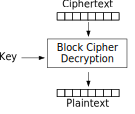
\includegraphics[width=4.5cm,height=3.5cm]{Decryption}
	 \end{minipage}
	\end{figure}
\end{frame}

\begin{frame}
\frametitle{structures of block ciphers}
	\begin{itemize}
		\item rounds
		\item feistel-network
		\item substitution-perumation-network
	\end{itemize}
\end{frame}

% ----

\begin{frame}
\frametitle{feistel-network}
	$L_{i+1} = R_i $ \\
	$R_{i+1} = L_i \oplus f(R_i, K_i)$
	\begin{center}
		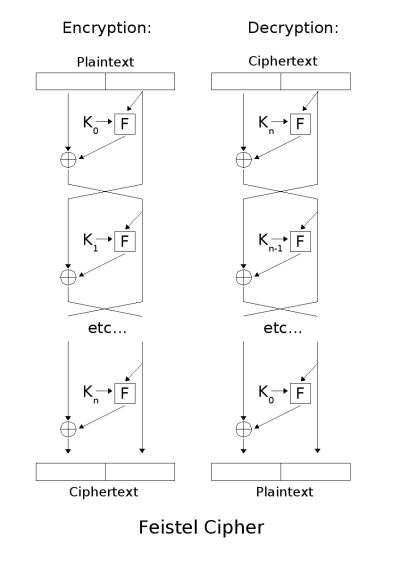
\includegraphics{Feistel}
	\end{center}
\end{frame}

% ----

\begin{frame}
\frametitle{S-Boxes}
	simple substituation function\\
	brings nonliearity\\
	mostly implemented as lookuptables
\end{frame}
